\section{Конструкторский раздел}
В данном разделе представлены диаграмма вариантов использования, диаграмма "сущность-связь"\ базы данных для хранения характеристик пользователя и IDEF0-диаграмма прикладной задачи определения усталости оператора АРМ.

\subsubsection{Включаемые в метод характеристики, получаемые с использованием периферийных устройств}

При проведении анализа метода распознавания усталости с использованием веб-камеры было указано, что применение данного метода может потребовать больших вычислительных ресурсов серверной части программного комплекса, а также постоянное соединение с сетью Интернет со стороны клиента. Данные факторы указывают на то, что метод не отвечает формализованным требованиям к прототипу метода систематического распознавания усталости на автоматизированном рабочем месте.

При проведении анализа метода распознавания усталости и стресса с использованием микрофона стало известно, что данный метод позволяет определить лишь проявления слабости, которые не могут однозначно указывать на наступление стадии истощения, адаптации или тревоги. Таким образом, метод не может быть включен в прототип метода систематического распознавания усталости на автоматизированном рабочем месте.

Для определения усталости будут использоваться устройства клавиатура и мышь. Для решения задачи будет построена нечеткая модель.

\subsubsection{Метод систематического распознавания усталости на автоматизированном рабочем месте}
Метод систематического распознавания усталости на автоматизированном рабочем месте включает в себя:
\begin{itemize}[leftmargin=1.6\parindent]
\item хранение и анализ данных, получаемых от клавиатуры --- для определения усталости используется нечеткая модель;
\item хранение и анализ данных, получаемых от мыши --- для определения усталости используется нечеткая модель.
\end{itemize}

Построение нечеткой модели происходит на этапе синхронизации поступающих данных о действия пользователя с данными о скорости его реакции в отдельные моменты времени. В дальнейшем данная модель используется до ее актуализации. Система актуализирует модель в случае, если будет определено, что имеют место ложные срабатывания и ``эталонные'' паттерны поведения субъекта изменились.

\subsection{Формат и метод сбора данных, предоставляемых оператором автоматизированного рабочего места}
В качестве данных, характеризующих действия оператора с клавиатурой и мышью, выступают нажатия клавиш клавиатуры и мыши, а также передвижения курсора мыши по экрану.

Каждое нажатие на клавишу клавиатуры характеризуется двумя полями:
\begin{itemize}[leftmargin=1.6\parindent]
\item наименование нажатой клавиши (в случае литеры --- литера, в случае специальных клавиш -- полное наименование);
\item временная метка, включающая в себя дату совершенного действия, и время в формате ЧЧ:ММ:СС.ССС, где Ч --- часы, М --- минуты, С --- секунды.
\end{itemize}

Каждое нажатие на клавишу мыши характеризуется четырьмя полями:
\begin{itemize}[leftmargin=1.6\parindent]
\item координата X, в которой было совершено действие;
\item координата Y, в которой было совершено действие;
\item номер нажатой кнопки мыши;
\item временная метка, включающая в себя дату совершенного действия, и время в формате ЧЧ:ММ:СС.ССС.
\end{itemize}

Передвижения курсора мыши характеризуется тремя полями:
\begin{itemize}[leftmargin=1.6\parindent]
\item координата X нового положения, в котором находится курсор;
\item координата Y нового положения, в котором находится курсор;
\item временная метка, включающая в себя дату совершенного действия, и время в формате ЧЧ:ММ:СС.ССС.
\end{itemize}

При беспрерывном передвижения курсора мыши по экрану его положения фиксируются каждые $\approx$ 0.010 секунд.

В качестве данных, формирующих нечеткую модель, используется тест на реакцию. Данный тест включает в себя появление некоторого элемента на экране и регистрацию времени, за которое оператор среагировал на его появление и нажал на него. При следующем появлении элемент не изменяет своей формы или положения, время появления элемента определяется случайным образом в интервале от двух до десяти секунд. Объекту предоставляется порядка десяти попыток, в результате чего среднее время реакции принимается за текущий показатель времени реакции пользователя. Тест проводится каждые 40 минут работы пользователя.

Может быть использован как локальный, так и удаленный метод сбора данных. Отличие данных методов заключается только в расположении хранилища данных. Первично данные должны записываться в логирующие файлы, которые в дальнейшем могут быть направлены в базу данных и удалены из локального хранилища.

Метод включает в себя логирование прерываний, поступающих с клавиатуры и мыши, включающих необходимую информацию о действиях пользователя, а также результатов тестов на реакцию.

\subsection{Диаграмма вариантов использования}
На рисунке \ref{fig:useCase} предоставлена диаграмма вариантов использования.
\begin{figure}[H]
	\centering
	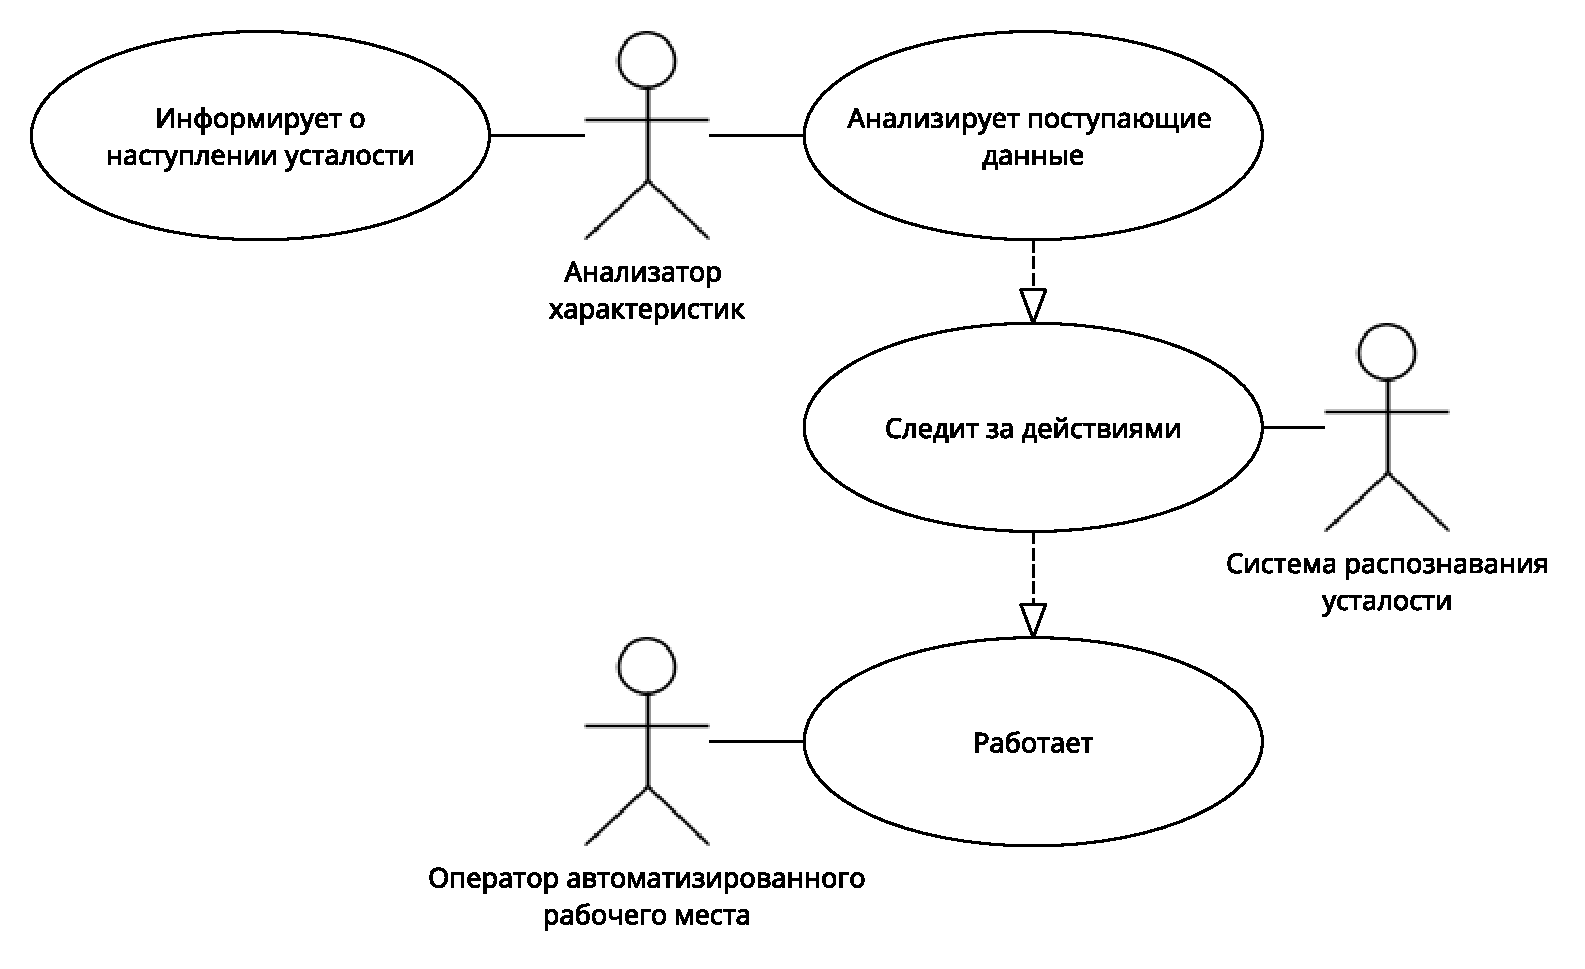
\includegraphics[width=\textwidth]{img/useCaseDiagram.pdf}
	\caption{Диаграмма вариантов использования.}
	\label{fig:useCase}
\end{figure}

В системе определены 3 роли: система распознавания усталости, анализатор характеристик и оператор автоматизированного рабочего места.

Роль системы распознавания усталости заключается в сборе и систематизации поступающей информации от оператора. Данная часть системы не анализирует информацию и определяется в качестве медиатора для базы данных и программного обеспечения снятия данных.

Анализатор поступающих характеристик формирует некоторую нечеткую модель по первичным данным, принимаемых за эталонных, а также отвечает за актуализацию участвующей в распознавании усталости модели. Также данная часть системы отвечает за информирование о наступлении усталости.

\subsection{IDEF0-диаграмма}
На рисунках \ref{fig:idef:0}--\ref{fig:idef:1} предоставлена диаграмма IDEF0 задачи определения усталости оператора АРМ.

\begin{figure}[H]
	\centering
	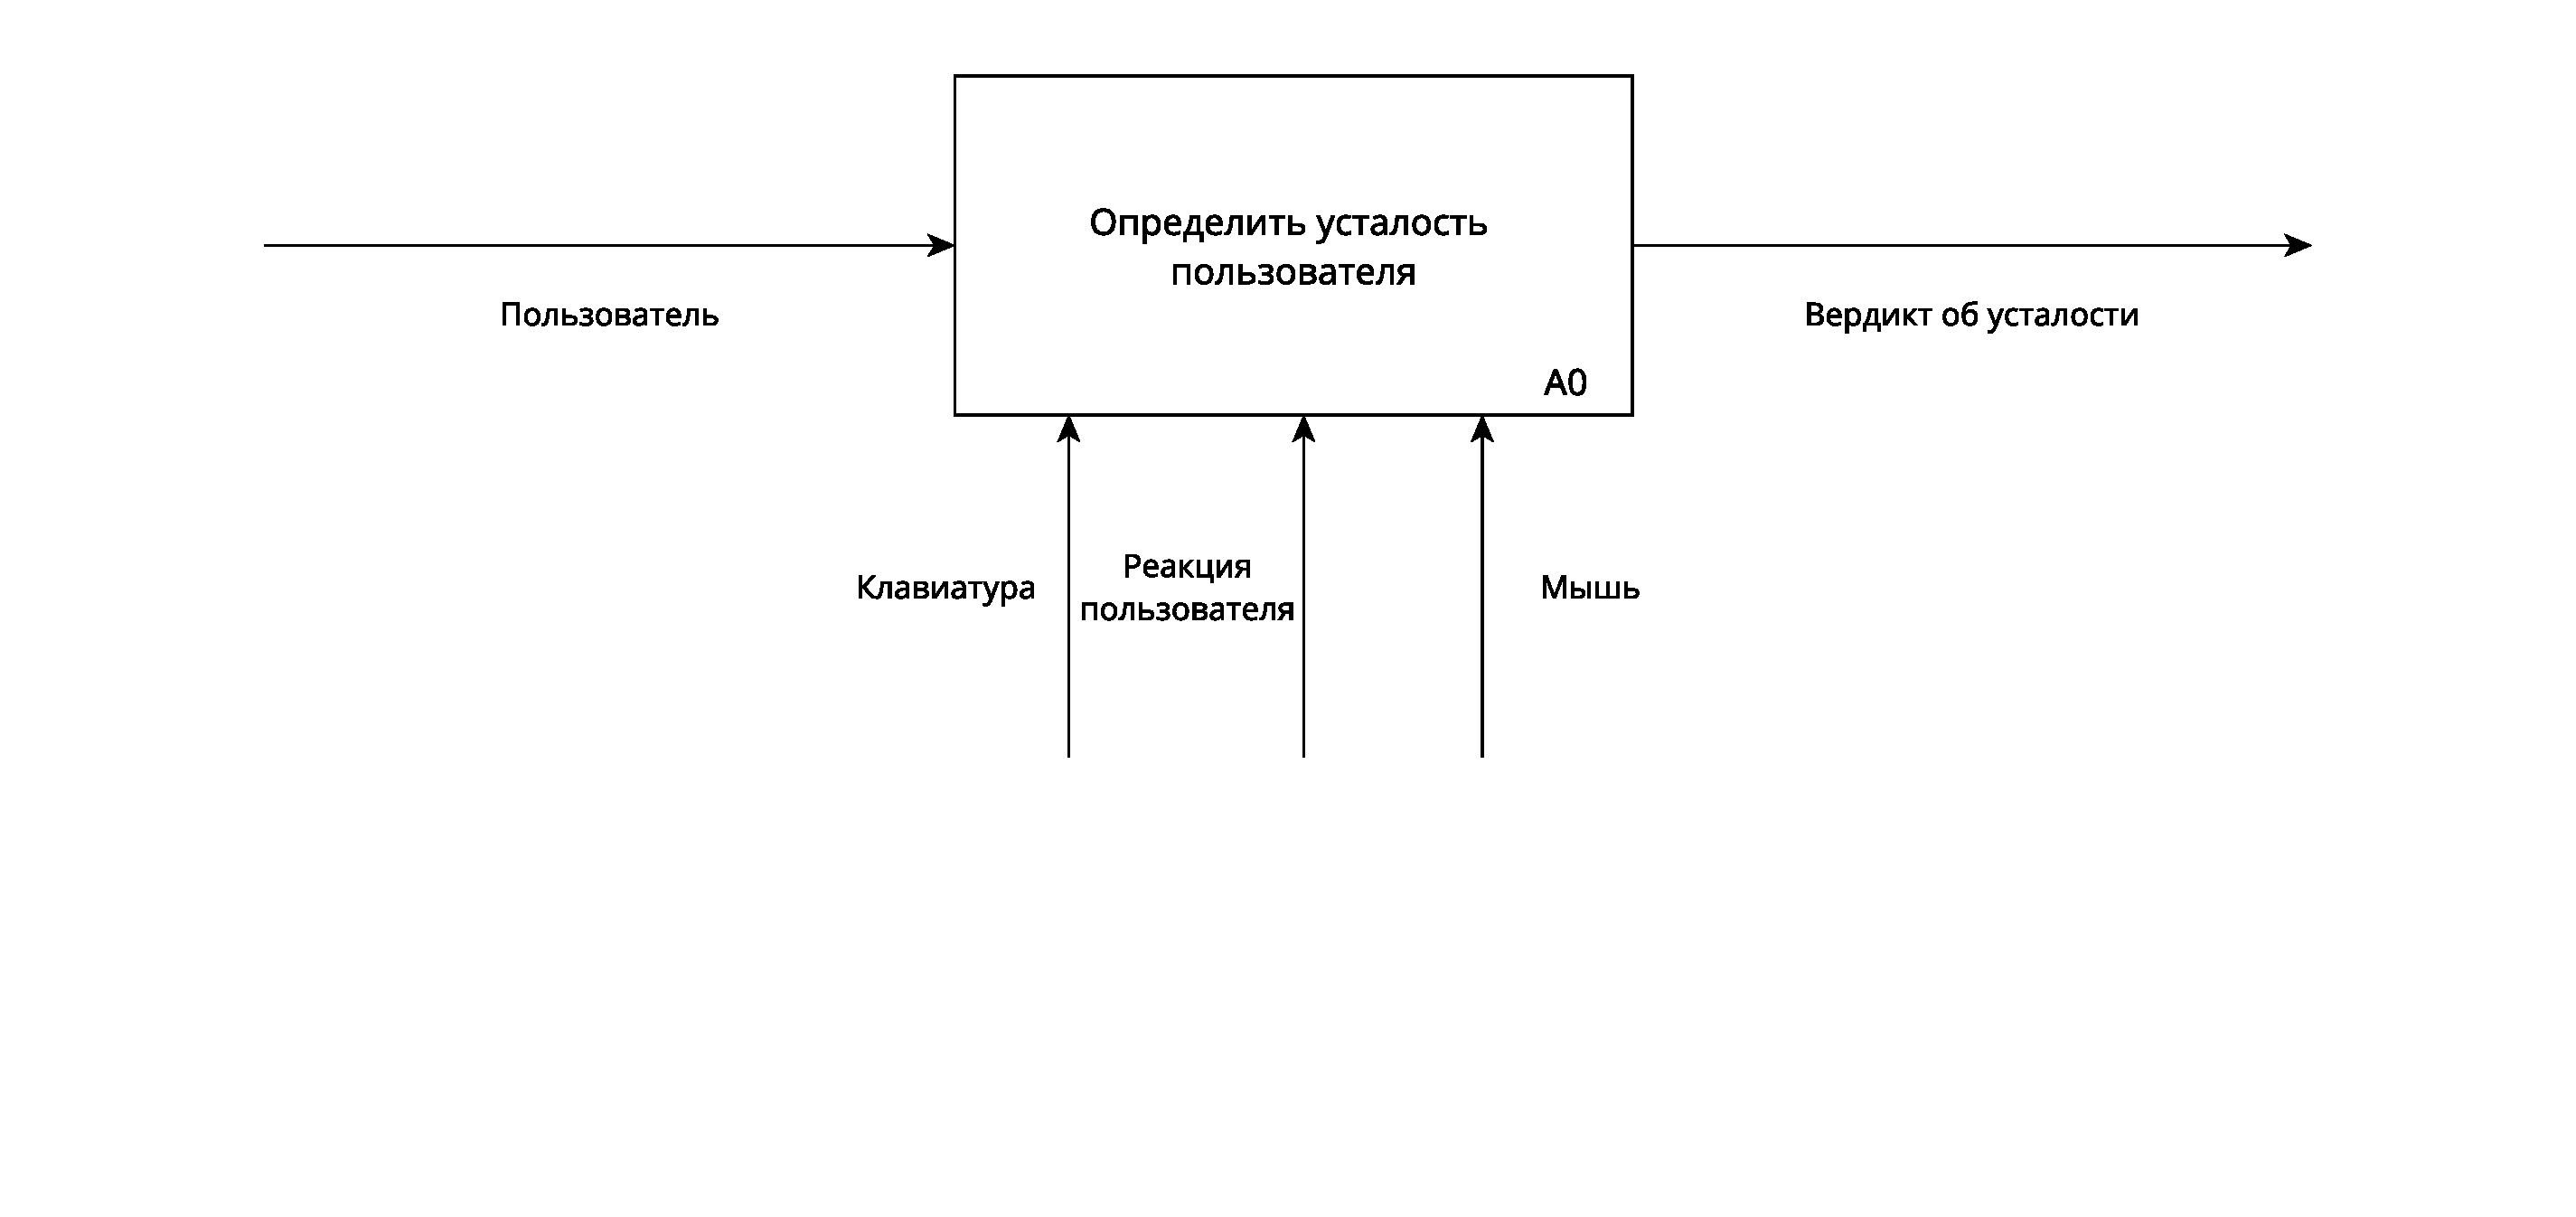
\includegraphics[width=\textwidth]{img/A0.pdf}
	\caption{IDEF0-диаграмма уровня A0.}
	\label{fig:idef:0}
\end{figure}

\begin{figure}[H]
	\centering
	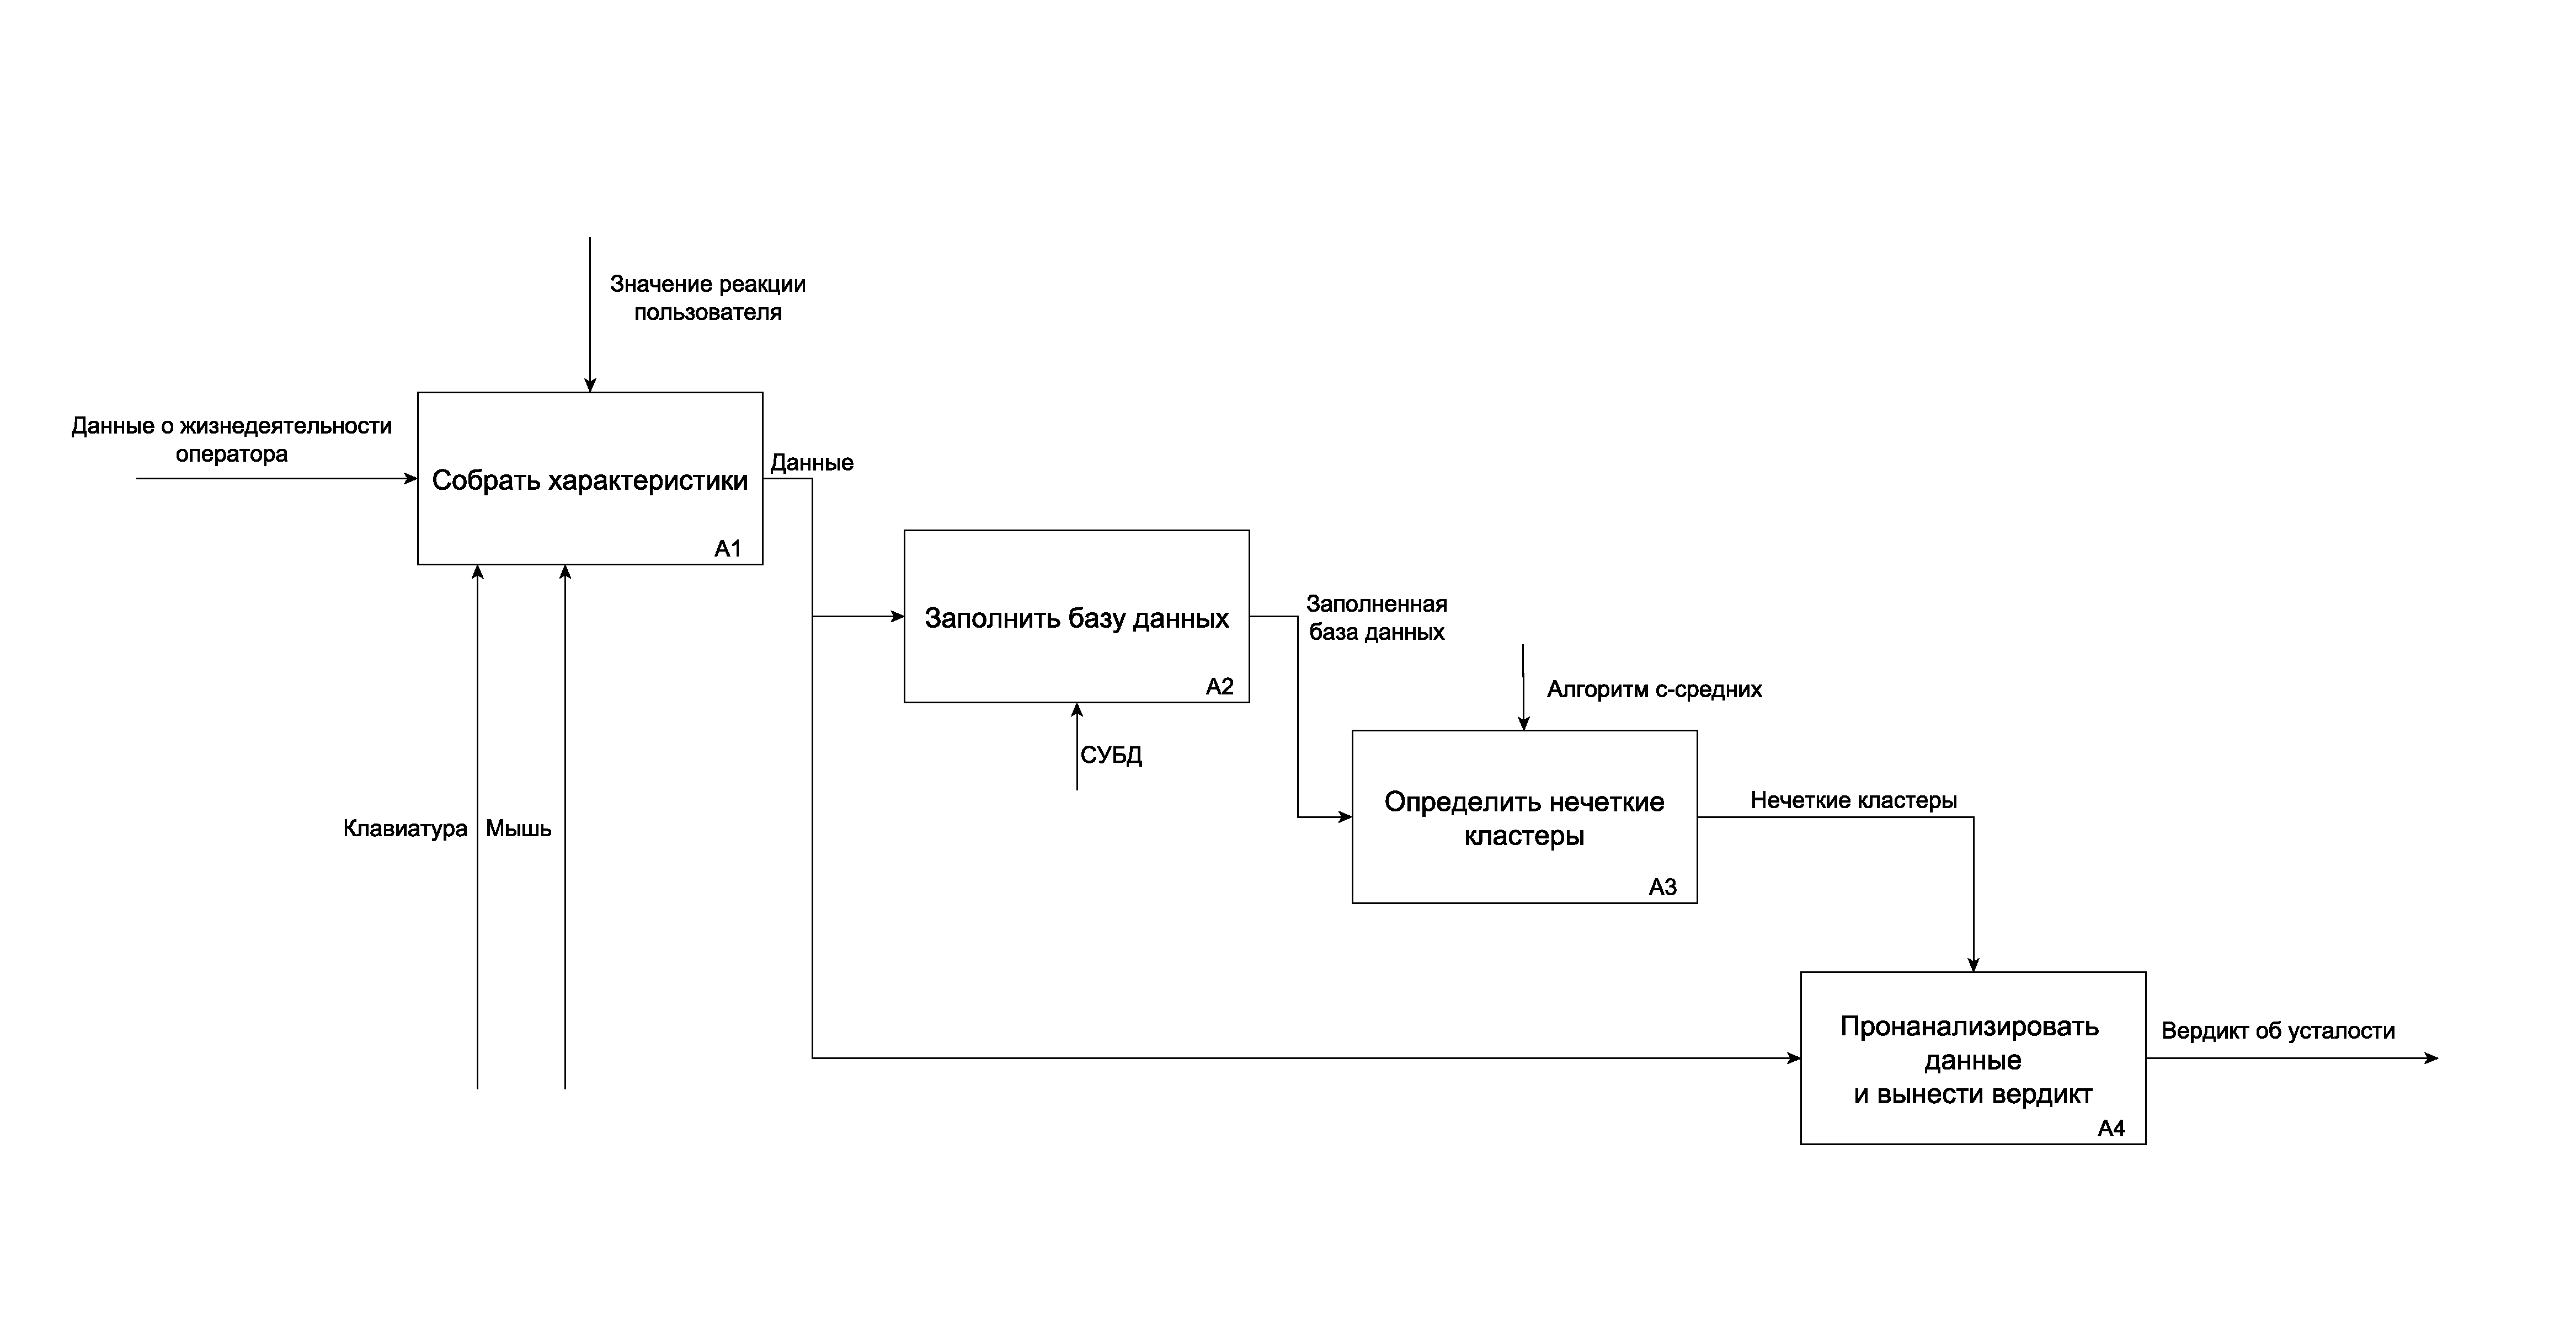
\includegraphics[scale=0.28]{img/A123.pdf}
	\caption{IDEF0-диаграмма уровня A1-A3.}
	\label{fig:idef:1}
\end{figure}

\subsection{Диаграмма ``сущность-связь'' в нотации Чена}
На рисунке \ref{fig:erDiag} предоставлена диаграмма ``сущность-связь'' в нотации Чена.

\begin{figure}[H]
	\centering
	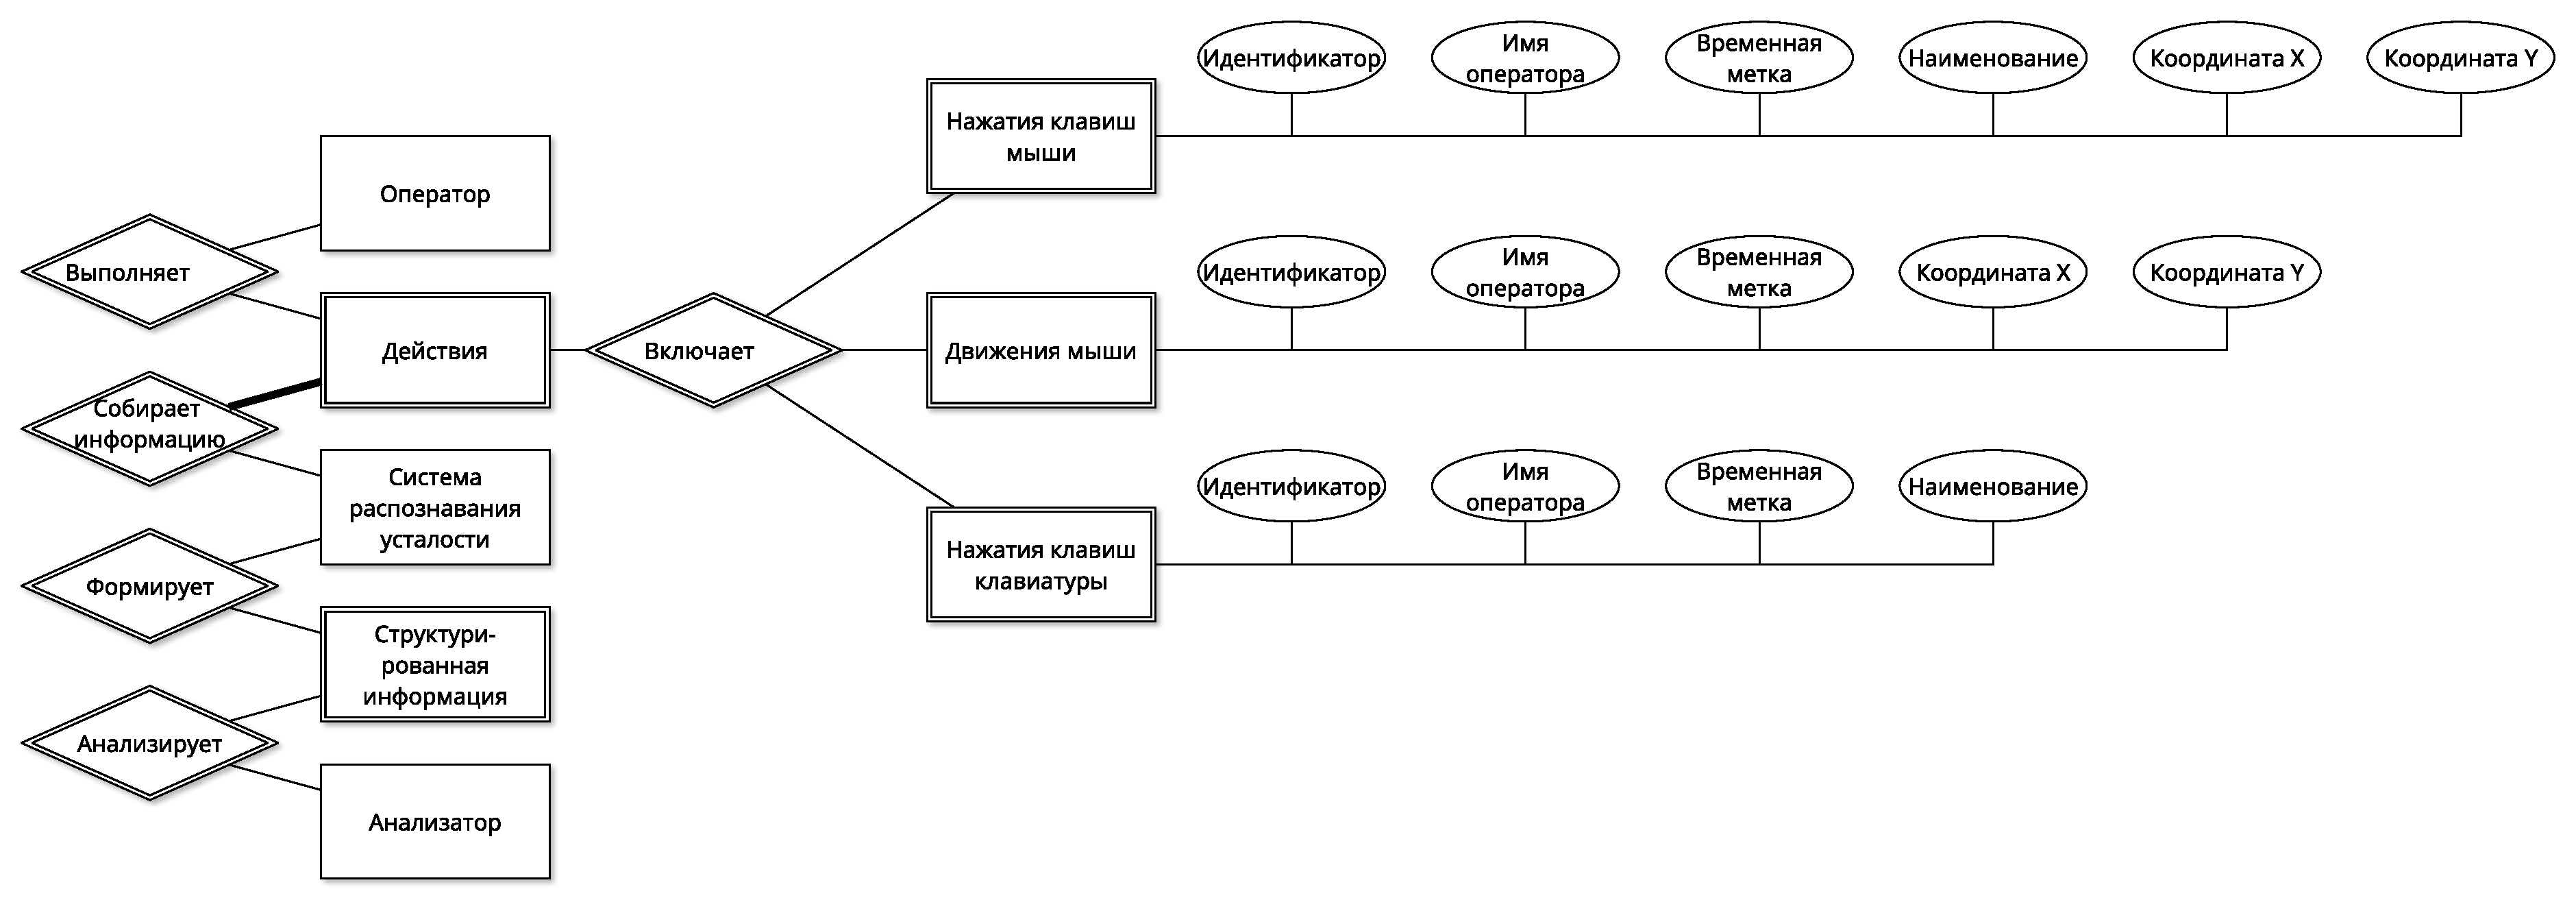
\includegraphics[scale=0.28]{img/chenERDiagram.pdf}
	\caption{Диаграмма ``сущность-связь'' в нотации Чена.}
	\label{fig:erDiag}
\end{figure}


\subsection{Используемые методы исследования корреляции}
Корреляционные методы позволяют решать задачи определения изменения зависимой переменной под влиянием одного или набора факторов, установки тесноты связи результативного признака с отдельным фактором, включенным в анализ. Также данные методы предоставляют возможность оценки общего объема вариации зависимой переменной и определения роли каждого фактора, а также проведения статистической оценки выборочных показателей корреляционной связи. \cite{correlInEco}

Характеристикой корреляционной зависимости является статистическая величина, называемая коэффициентом корреляции. \cite{corelMethod}

\subsubsection{Парная корреляция}

Для парной корреляции (фактор и отклик имеют нормальные распределения), коэффициент корреляции вычисляется по формуле \cite{corelMethod}:

\begin{equation}
\label{eq:corelPara}
\rho = \frac{M\left \{\left[x-M\left(X\right)\right]\left[y-M(Y)\right]\right \}}{\sqrt{M\left[x-M\left(X\right)^2\right]M\left[y-M\left(Y\right)^2\right]}} = \frac{K_{XY}}{\sqrt{D\left(X\right)D\left (Y\right)}},
\end{equation}
\eqexplSetIntro{где}
\begin{eqexpl}[15mm]
\item{$K_{XY}$} корреляционный момент, представляющий собой математическое ожидание произведения отклонений значений $x$ и $y$ случайных величин $X$ и $Y$ от их математических ожиданий $M(X)$ и $M(Y)$;
\item{$D(X)$} дисперсия случайной величины $X$;
\item{$D(Y)$} дисперсия случайной величины $Y$.
\end{eqexpl}

На практике случайные величины представляются ограниченным числом значений, поэтому вместо значения коэффициента корреляции $\rho$ используется его оценка $r$, которая рассчитывается с использованием выборочных характеристик отклика и фактора \cite{corelMethod}:

\begin{equation}
\label{eq:corelMark}
r = \frac{\sum_{i = 1}^{n}(x_i - \overline{x})(y_i - \overline{y}))}{(n - 1)\overline{S}_X \overline{S}_Y},
\end{equation}
\eqexplSetIntro{где}
\begin{eqexpl}[20mm]
\item{$\overline{x}$ и $\overline{y}$} средние выборочные значения фактора и отклика;
\item{$\overline{S}_X$ и $\overline{S}_Y$} выборочные стандартные отклонения отклика и фактора;
\item{$n$} число наблюдений.
\end{eqexpl}

Следует отметить, что значение $r$ лежит на интервале от $-1$ до $+1$. В случае, когда $r=\pm1$ зависимость между фактором и откликом является функциональной. Также положительное значение коэффициента корреляции указывает на возрастание отклика с увеличением фактора, когда отрицательные значение свидетельствует об убывании $Y$ при возрастании $X$. Равенство коэффициента парной корреляции нулю указывает, что взаимосвязь не является линейной. \cite{corelMethod}

\subsubsection{Множественная корреляция}
Множественная корреляция определяет обусловленность некоторого признака одновременным действием нескольких других признаков. Взаимодействия отклика с каждым из факторов и факторов между собой отображают в виде матрицы корреляции. \cite{corelMethod}

\begin{table}[H]
\begin{center}
\caption{\label{table: corelMatrix} Матрица корреляции}
\begin{tabular}{l||llllll}
      & $Y$         & $X_1$         & $...$ & $X_j$          & $...$ & $X_m$             \\ \hline\hline
$Y$   & $1$         & $r_{Y,X_1}$   & $...$ & $r_{Y,X_j}$    & $...$ & $r_{Y,X_m}$    \\
$X_1$ & $r_{Y,X_1}$ & $1 $          & $...$ & $r_{X_1,X_j}$  & $...$ & $r_{X_1,X_m}$ \\
$...$ & $...$       & $...$         & $1$   & $...$          & $...$ & $...$              \\
$X_j$ & $r_{Y,X_j}$ & $r_{X_1,X_j}$ & $...$ & $1$            & $...$ & $r_{X_m,X_m}$ \\
$...$ & $...$       & $...$         & $...$ & $...$          & $1$   & $...$              \\
$X_m$ & $r_{Y,X_m}$ & $r_{X_1,X_m}$ & $...$ & $r_{X_j,X_m}$  & $...$ & $1$               
\end{tabular}
\end{center}
\end{table}

Коэффициент множественной корреляции определяют из предположения, что отклик связан с факторами линейной зависимостью, причём коэффициент вычисляется по следующей формуле:
\begin{equation}
\label{eq:fuckMark}
R = \sqrt{1 - \frac{\Delta_{YX}}{\Delta_{XX}}},
\end{equation}
\eqexplSetIntro{где}
\begin{eqexpl}[15mm]
\item{$\Delta_{YX}$} определитель матрицы корреляции;
\item{$\Delta_{XX}$} определитель матрицы, получаемой из матрицы корреляции вычеркиванием первой строки и первого столбца.
\end{eqexpl}

Значимость множественного коэффициента корреляции проверяется с импользованием критерия Фишера:

\begin{equation}
\label{eq:fisherCrit}
F_\rho = \frac{R^2}{1-R^2} \frac{n - m - 2}{m} > F\left[{\alpha;m;n-m-2}\right],
\end{equation}
\eqexplSetIntro{где}
\begin{eqexpl}[60mm]
\item{$F_\rho$ и $F\left[\alpha;m;n-m-2\right]$} рассчитаное и табличное числа Фишера.
\end{eqexpl}

При выполнении условия \eqref{eq:fisherCrit} коэффициент множественной корреляции можно считать значимым с доверительной вероятностью $p = 1 - \alpha$.

\subsection{Используемые методы дисперсионного анализа}

Дисперсионный анализ позволяет определить, влияет ли некоторый фактор или группа факторов на изучаемую величину, какой из них имеет наибольшее влияние, а также зависит ли влияние факторов от их взаимодействия друг с другом. \cite{disperMethod}

\subsubsection{Однофакторный дисперсионный анализ}
Некоторый фактор $A$ имеет $m$ уровней и число $y_{ij}$ получено в результате $j$-го опыта, проведенного на его $i$-м уровне. Числа $y_{ij}$ --- это наблюдения, а $n_i$ --- число наблюдений, полученных на i-м уровне. Наблюдения представляются в виде \cite{disperMethod}:

\begin{equation}
\label{eq:watcha}
y_{ij} = \mu_i+\varepsilon_{ij},
\end{equation}
\eqexplSetIntro{где}
\begin{eqexpl}[15mm]
\item{$\mu_i$} математическое ожидание $y$ на $i$-ом уровне;
\item{$\mu_{ij}$} случайная ошибка.
\end{eqexpl}

Если фактор не влияет на переменную $y$, то рассеяние ее значений вызывается лишь случайными ошибками, а математические ожидания на всех уровнях одинаковы. \cite{disperMethod}

Обозначим $\alpha_i=\mu_i-\mu, \mu=\frac{1}{n}\sum_{i=1}^{m}{n_i\mu_i}$. Значение $\alpha$ называется эффектом фактора $A$ на уровне $i$. Таким образом уравнение \eqref{eq:watcha} примет вид \cite{disperMethod}:

\begin{equation}
\label{eq:watcha}
y_{ij} = \mu+\alpha_i+\varepsilon_{ij},
\end{equation}


Следующие рассуждения строятся на предположении о том, что случайные ошибки имеют нулевое математическое ожидание, постоянную дисперсию и подчиняются нормальному распределению.

Определяются следующие величины:

\begin{equation}
\label{eq:yig}
y_{ig}=\frac{1}{n_i}\sum_{j=1}^{n_i}{y_{ij}},
\end{equation}
\begin{equation}
\label{eq:eij}
e_{ij}=y_{ij}-y_{ig},
\end{equation}
\begin{equation}
\label{eq:ygg}
y_{gg}=\frac{1}{n}\sum_{i,j}{y_{ij}},
\end{equation}
\begin{equation}
\label{eq:alphai}
\widehat{\alpha}_i=y_{ij}-y{gg},
\end{equation}
\eqexplSetIntro{где}
\begin{eqexpl}[15mm]
\item{$y_{ig}$} средние значения по столбцам;
\item{$e_{ij}$} отклонения от среднего в каждом столбце;
\item{$y_{gg}$} общее среднее, $n=\sum_{i=1}^{m}{n_i}$;
\item{$\widehat{\alpha}_i$} отклонения средних по столбцам от общего среднего.
\end{eqexpl}

Можно доказать, что:

\begin{equation}
\label{eq:meij}
M(e_{ij})=0,M(y_{gg})=\mu,M(\widehat{\alpha}_i)=\mu_i-\mu=\alpha_i, \mu=\frac{1}{n}\sum_{i=1}^{m}{n_i\mu_i},
\end{equation}

Соотношения \eqref{eq:meij} означают, что случайные величины $y_{ig}$ и $\widehat{\alpha}_i$ являются несмещенными оценками параметров $\mu_i$ и $\alpha_i$.

Справедливо соотношение:

\begin{equation}
\label{eq:spsum}
S_П=S_М+S_В,
\end{equation}

Причем:

\begin{equation}
\label{eq:sp}
S_П=\sum_{i,j}{\left(y_{ij}-y_{gg}\right)^2},
\end{equation}
\eqexplSetIntro{где}
\begin{eqexpl}[15mm]
\item{$S_П$} Полная сумма квадратов.
\end{eqexpl}

\begin{equation}
\label{eq:sp}
S_М=\sum_{i=1}^{m}{n_i\left(y_{ij}-y_{gg}\right)^2=\sum_{i=1}^{m}{n_i\widehat{\alpha}_i^2}},
\end{equation}
\eqexplSetIntro{где}
\begin{eqexpl}[15mm]
\item{$S_М$} межгрупповая сумма квадратов, характеризующая рассеяние средних по столбцам относительно общего среднего.
\end{eqexpl}

\begin{equation}
\label{eq:sv}
S_В=\sum_{i,j}{\left(\left(y_{ij}-y_{ig}\right)^2\right)},
\end{equation}
\eqexplSetIntro{где}
\begin{eqexpl}[15mm]
\item{$S_В$} внутригрупповая сумма квадратов, характеризующая рассеяние значений $y_{ij}$ относительно $y_{ig}$, то есть рассеяние внутри групп.
\end{eqexpl}

Если гипотеза верна и $\alpha_1=\alpha_2=...=\alpha_m=0$, то величины $\widehat{\alpha}_i$ должны быть достаточно близки к нулю. Тогда вклад $S_М$ и $S_П$ по сравнению с $S_В$ должен быть мал. Поэтому малое значение $S_М$ является доводом в пользу гипотезы, а большое значение $S_М$ является доводом против гипотезы. Точный метод проверки гипотезы основан на F-критерии. \cite{disperMethod}

\subsubsection{Двухфакторный дисперсионный анализ с однократными наблюдениями}
В данном методе рассматривается возможное влияние нескольких факторов на некоторую переменную $y$.

При изучении факторов $A$ и $B$ на переменную $y$ можно представить модель в виде:
\begin{equation}
\label{eq:modelTwoFactors}
y_{ij}=\mu_{ij}+\varepsilon_{ij},i=1,...,I;j=1,...,J,
\end{equation}
\eqexplSetIntro{где}
\begin{eqexpl}[15mm]
\item{$\mu_{ij}$} некоторые константы;
\item{$\varepsilon_{ij}$} случайные ошибки;
\item{$I,J$} число уровней факторов $A$ и $B$ соответственно;
\item{$y_{ij}$} наблюдение, полученное на $i$-м уровне фактора $A$ и на $j$-м уровне фактора $B$.
\end{eqexpl}

Случайные ошибки также должны удовлетворять требованиям, что и в однофакторном случае.

Если между факторами отсутствует взаимодействие, то влияние одного фактора на величину $y$ не зависит от того, на каком уровне находится другой фактор. От Таким образом уравнение \eqref{eq:modelTwoFactors} можно записать в следующем виде:

\begin{equation}
\label{eq:newModel}
y_{ij}=\mu+\alpha_i+\beta_j+\varepsilon_{ij}, i=1...,I;j=1,...,J,
\end{equation}
\eqexplSetIntro{где}
\begin{eqexpl}[15mm]
\item{$\mu$} общее среднее;
\item{$\alpha_i$} эффект фактора $A$ на его $i$-ом уровне;
\item{$\beta_j$} эффект фактора $B$ на его $j$-м уровне.
\end{eqexpl}

Для проверки предположения о том, что фактор $A$ или $B$ не влияет на переменную $y$ потребуется проверить гипотезы о равенстве нулю соответствующих эффектов:

\begin{equation}
\label{eq:hyposForNewModel}
H_A:\alpha_i=0,i=1,...,I, H_B:\beta_j=0,j=1,...,J,
\end{equation}

Для этого потребуется вычислить величины:

\begin{equation}
\label{eq:yignew}
y_{ig}=\frac{1}{J}\sum_{j=1}^{J}{y_{ij}},
\end{equation}
\eqexplSetIntro{где}
\begin{eqexpl}[15mm]
\item{$y_{ig}$} средние по строкам.
\end{eqexpl}

\begin{equation}
\label{eq:ygjnew}
y_{gj}=\frac{1}{I}\sum_{i=1}^{I}{y_{ij}},
\end{equation}
\eqexplSetIntro{где}
\begin{eqexpl}[15mm]
\item{$y_{gj}$} средние по столбцам.
\end{eqexpl}

\begin{equation}
\label{eq:yggnew}
y_{gg}=\frac{1}{IJ}\sum_{i,j}{y_{ij}},
\end{equation}
\eqexplSetIntro{где}
\begin{eqexpl}[15mm]
\item{$y_{gg}$} общее среднее.
\end{eqexpl}

Далее вычисляются значение $\widehat{\alpha}_i = y_{ig}-y_{gg}$ и $\widehat{\beta}_j=y_{gj}-y_{gg}$. Эти величины являются несмещенными оценками соответствующих параметров. Если гипотезы верны, то данные оценки не должны значимо отличаться от нуля. Алгоритм проверки основан на критерии Фишера, как и в предыдущем варианте. \cite{disperMethod}

\subsection{Алгоритмы кластеризации}
Задачей кластеризации является объединение в группы объектов, схожих по некоторому признаку. Данная задача включает в себя разбиение множества объектов, называемых кластерами. \cite{clasters}

Одним из главных отличий кластеризации от классификации является факт того, что перечень групп четко не задан и определяется в процессе работы алгоритма. \cite{clasters}

Этапы кластерного анализа включают в себя \cite{clasters}:

\begin{itemize}[leftmargin=1.6\parindent]
\item отбор выборки объектов;
\item определение множества переменных, по которым будут оцениваться объекты в выборке;
\item вычисление значений меры сходства между объектами;
\item применение метода кластерного анализа;
\item представление результатов анализа.
\end{itemize}

Выделяют две основные классификации алгоритмов кластеризации: иерархические и плоские и четкие и нечеткие. \cite{clasters}

Иерархические алгоритмы строят не одно разбиение выборки на непересекающиеся кластеры, а систему вложенных разбиений. Плоские алгоритмы Строят разбиение объектов на кластеры. \cite{clasters}

Четкие алгоритмы каждому объекту выборки ставят в соответствие номер кластера, то есть каждый объект определенно относится к одному из выделенных кластеров. Нечеткие алгоритмы каждому объекту ставят в соответствие набор вещественных значений, показывающих степень отношения объекта к кластерам, каждый объект относится к каждому кластеру с некоторой вероятностью. \cite{clasters}

\subsubsection{Алгоритмы иерархической кластеризации}

Среди алгоритмов иерархической кластеризации выделяются два типа: нисходящие и восходящие алгоритмы. В первом типе в начале все объекты помещаются в один кластер, который затем разбивается на все более мелкие кластеры. Восходящие алгоритмы в начале работы помещают каждый объект в отдельный кластер, а затем объединяют кластеры во все более крупные, пока все объекты выборки не будут содержаться в одно кластере. \cite{clasters}

\subsubsection{Нечеткие алгоритмы}
Наиболее популярным алгоритмом нечеткой кластеризации является алгоритм c-средних. Он представляет собой модификацию метода k-средних. \cite{clasters}

Алгоритм может быть описан следующей последовательностью действий \cite{clasters}:

\begin{itemize}[leftmargin=1.6\parindent]
\item Выбрать начальное нечеткое разбиение n объектов на k кластеров путем выбора матрицы принадлежности U размера (n, k);
\item используя матрицу U, найти значение критерия нечеткой ошибки:

вставить формулу;
\item Перегруппировать объекты с целью уменьшения этого значения критерия нечеткой ошибки;
\item Возвращаться в п. 2 до тех пор, пока изменения матрицы U не станут незначительными.
\end{itemize}

Данный алгоритм может не подойти, если заранее неизвестно число кластеров, либо необходимо однозначно отнести каждый объект к одному кластеру.

Привести еще к-средних, выделение связных компонент и в конце привести таблицу такую же, как и у них.

\subsection*{Вывод}
Юрий Владимирович запретил мне работать на стройке

\pagebreak